\documentclass[]{standalone}
%\usepackage{mathptmx}
%\renewcommand{\familydefault}{\rmdefault}
\usepackage[T1]{fontenc}
\usepackage[latin9]{inputenc}
\usepackage{siunitx}
\usepackage{array}
\usepackage{amsmath}
\usepackage{ifthen}
\usepackage{pgfplots}
\pgfplotsset{compat=1.14}
\usepackage{titling, graphicx}
\usepackage{tikz}
\usepackage{upgreek}
\usepackage{amsmath,amsthm}
\usepackage{strtikz}
\usetikzlibrary{shapes,arrows.meta,intersections,graphs,graphs.standard}
\usetikzlibrary{bending, math,fit}
\usetikzlibrary{calc,intersections,through,backgrounds,decorations.pathmorphing}
%\usetikzlibrary{fpu}
%\usepackage{pgfmath}


\begin{document}


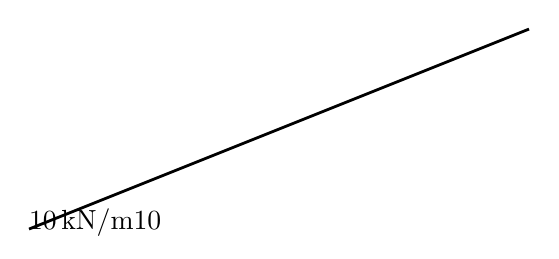
\begin{tikzpicture}
\draw [line width=1](0, 0) -- (2.5in, 1in);
\frametriangularload[startx = 0cm,
starty = 0cm,
endx = 2.5in,
endy = 1in,
number of arrows = 10,
print first arrow = 0,
height of arrows left= 0cm,
height of arrows right= 2.cm,
space = 0.0cm,
start ratio = 0.025,
end ratio = 0.025,
right load text = $\SI{10}{\kilo\newton/\meter}$,
left load text = $10$,
right text shiftx=0pt,
right text shifty=5pt,
left text shiftx=-10pt,
left text shifty=5pt,
arrow length=5pt,
arrow width=3pt,
arrow scale=1,
arrow line thickness=1pt]
%$\SI{10}{\kilo\newton/\meter}$
\end{tikzpicture}


\end{document}